% Licensed to the Apache Software Foundation (ASF) under one or more
% contributor license agreements. See the NOTICE file distributed with
% this work for additional information regarding copyright ownership.
% The ASF licenses this file to You under the Apache License, Version 2.0
% (the ``License''); you may not use this file except in compliance with
% the License. You may obtain a copy of the License at
%
% http://www.apache.org/licenses/LICENSE-2.0
%
% Unless required by applicable law or agreed to in writing, software
% distributed under the License is distributed on an ``AS IS'' BASIS,
% WITHOUT WARRANTIES OR CONDITIONS OF ANY KIND, either express or implied.
% See the License for the specific language governing permissions and
% limitations under the License.

\subsubsection{Configuring a Livelink Authority Connection}

The following options are specific to Livelink:

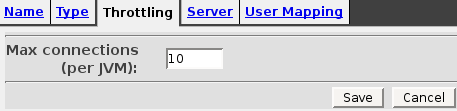
\includegraphics[width=300pt]{edit-authority-tab3}

\begin{itemize} 

\item \textbf{Max Connections (per JVM):} Here you can specify a
maximum number of connections for your authority
connection. \ifCombinedConnectorGuide The maximum number of
connections can affect system licensing and performance. See the Max
Connections item on page \pageref{max-auth} for more details.\fi

\ifLivelinkGuide
The maximum number of connections per JVM is important for two reasons.
First, the number of connections may impact the licensing on your document
server, depending on the repository. If you have a finite number of
Livelink connections available, they will be split between the authority
connector, which authorizes user access to documents, and the repository
connector, which actually downloads the documents to the appliance.

Second, the number of connections may impact the resources
available on the appliance. If the connector framework is slowing down
your appliance, lowering this number should help.
\fi

\end{itemize}

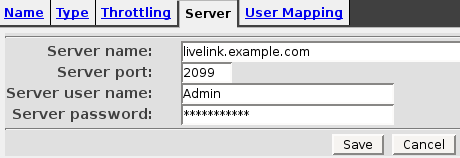
\includegraphics[width=300pt]{edit-authority-tab4}

\begin{itemize}

\item \textbf{Server name:} The name of the Livelink server from which
you wish to get authorization information.

\item \textbf{Server port:} The port on the Livelink server to which you
should connect. If you don't know what value this should be, ask your
Livelink administrator.

\item \textbf{Server user name:} The username you were given by your
Livelink administrator for connecting to the server. (The user account
must have sufficient authority to retrieve file ACLs.)

\item \textbf{Server password:} The password you were given by your
Livelink administrator for the above username.

\end{itemize}

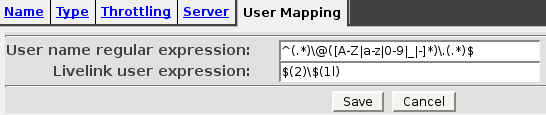
\includegraphics[width=300pt]{edit-authority-tab5}

\begin{itemize}

\label{regex}
\item \textbf{User name regular expression:} In many cases, the username
that an end-user will authenticate to GTS with is not the same as the
username that the Livelink server expects. This regular expression is used
to break the incoming username into pieces that can then be processed by
the next regular expression to produce a proper Livelink user name. The
default regular expression, \\ \verb+(.*)\@([A-Z|a-z|0-9|_|-]*)\.(.*)+,
separates an Active Directory \\ username of the form USER@DOMAIN.COM
into three distinct portions: USER, DOMAIN, and COM. In many cases,
this expression will be sufficient for you.

\note{If you are not familiar with regular expressions, there
are a variety of tutorials available on the web, including
\url{http://gnosis.cx/publish/programming/regular_expressions.html}
and \url{http://perldoc.perl.org/perlrequick.html}. If you still have
difficulty with these settings, please contact Customer Support (see
page \pageref{SupportContact}).}

\item \textbf{Livelink user expression:} Once you have deconstructed
the Active Directory username, you need to put it back together as an
appropriate Livelink username for your site's Livelink instance. The
default is the expression \verb+$(2)\$(1l)+, which takes the second value
from the first regular expression (DOMAIN), adds a backslash
(\verb+\+), and then puts the first value from the first expression in
place in lowercase (user), producing \verb+DOMAIN\user+. Depending on
how your Livelink instance is configured, you may need to change this
value. 

This expression may contain either plain text or variable expressions
such as \verb+$(2)+ above.  A variable expression, which must be of
the form \verb+$(N)+ where N is a number, represents a string from the
regular expression defined previously. You can force the string to be
all uppercase or lowercase by appending a \verb+u+ or \verb+l+ to the
string number. For example, to make the third string all in uppercase,
you would use \verb+$(3u)+. A dollar sign character must be escaped
with another dollar sign before it, so \verb+$$+ in this text box will
produce \verb+$+ in the user expression.

\end{itemize}

After entering this information, you will be taken to the authority
connection status page for this authority:

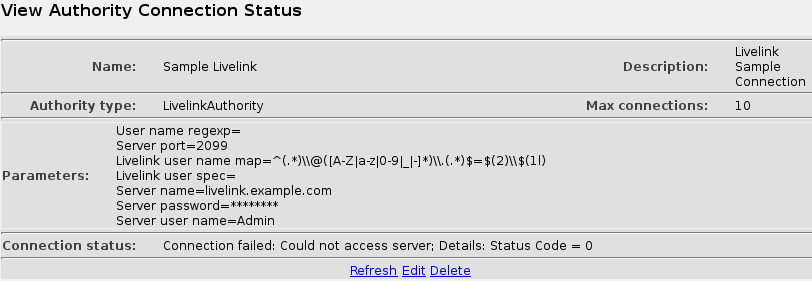
\includegraphics[width=300pt]{view-auth-conn-status}

In this example (which does not contain accurate information for any
Livelink server), the Connection Status is ``Connection failed.''
If you see this message, you most likely have incorrectly entered one
of the fields, and should click ``Edit'' to fix the data. If you have
entered everything as you intended, please inform your Livelink administrator;
you may not have been given the correct information.

